

\section{Селективное лазерное спекание}
\subsection{Технология}
Процесс печати изделия изображен схематически на рис. \ref{fig:printer}.\\
Описание. 


\begin{figure}[h]
    \centering
    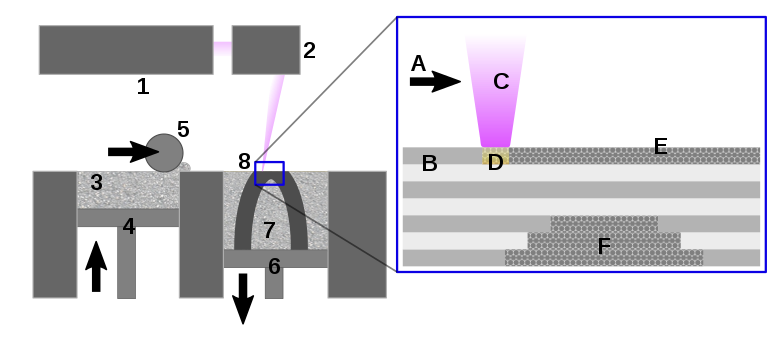
\includegraphics[width=\linewidth]{fig/sls.png}
    \caption{Caption}
    \label{fig:printer}
\end{figure}
анизотропия, слои\\
чтоб успевало спекаться (не спалвляться!!!)\\
Спекание отличается о сравнения

\subsection{Модель}

The high intensity of
the laser beam makes it possible to rapidly heat a small
region, inducing a disequilibrium of the temperature
distribution and large temperature gradients.\cite{sls-sim2016}
\\
The simulation
results showed a big difference in the temperature distributions
of composite powders, especially in terms of melting depth.\\
The experimental investigation became more
efficient due to the process predictions. The accuracy of the model
was validated by the microstructures of PA, PA/CF and PA/NaCl.
With the increasing research into various composites, this numerical
method can be further used to adopt appropriate processing
parameters for the production of functional parts and then engender
significant time and material savings.
\section{Характеристиики полимеров для СЛС}

The properties of the final product obtained by the SLS technology largely depend on the properties of the original powder (morphology, size, size distribution, bulk density, thermal properties, viscosity and surface tension) and on the parameters of laser sintering (laser power, scanning speed, laser spot diameter). Particle morphology affects the spatial arrangement of powder particles (stacking degree) relative to each other. Spherical (with a smooth surface) particles have a high packing density. They provide flowability of the powder composition in systems of applying the material with minimal resistance. In addition, spherical particles are well bonded in the process of laser sintering. It was shown that during the transition from powder particles with predominantly spherical morphology to particles of irregular shape of the same material, the elastic modulus decreases by almost 40 \%.3 The spherical particles with good flowability and a high packing densities represent ideal characteristics of the starting powder for use in SLS.4 At the same time, the use of irregularly shaped particles with a large variation in their size leads to the creation of products with higher mechanical characteristics, compared to the use of mainly spherical particles with a narrow size distribution.5

\subsection{Тепловые и механические параметры}
первая глава из
\cite{termopols}


\subsection{"Тонкая" Структура}
Что ее характеризует


\subsection{Полиэфиримиды ряда R-BAPB }
		
	\begin{figure}[h]
	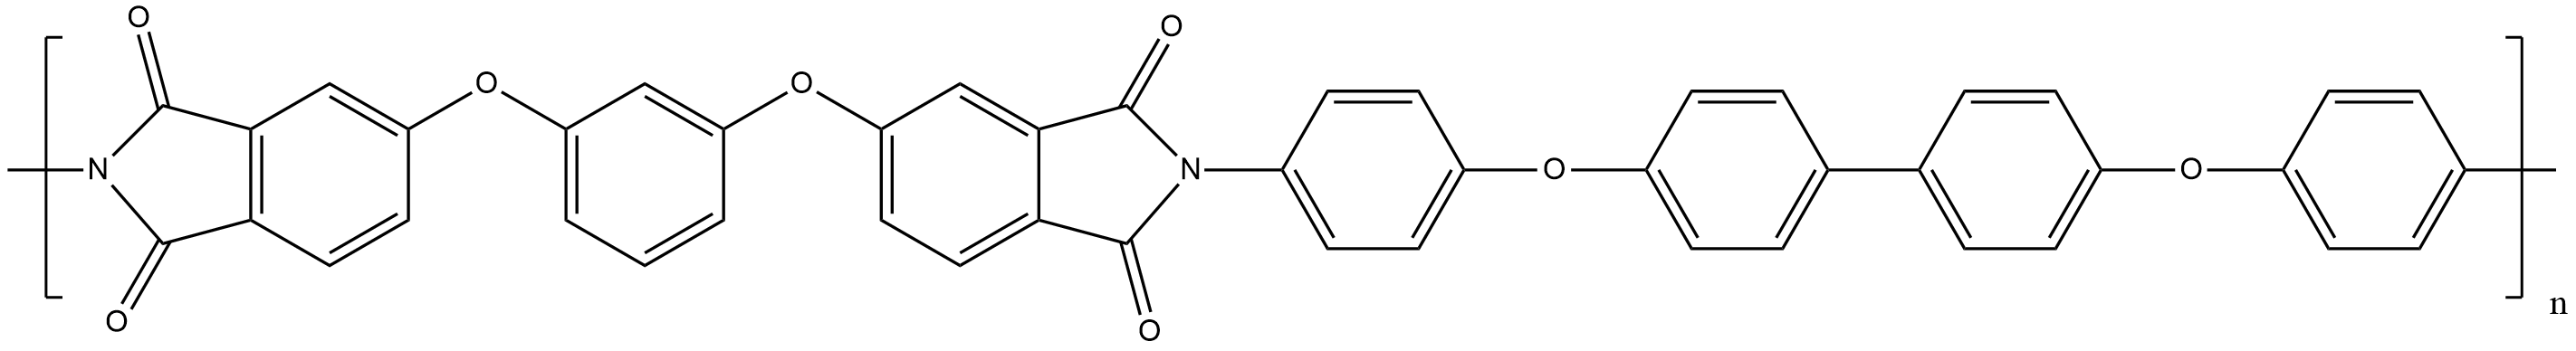
\includegraphics[width=\textwidth]{fig/formula.png}
	\end{figure}
	структура

Что следует из первичной структуры, термостойкость, особенности, пригодность для СЛС, перспективность

Данные по композитным добавкам

характеристики - все что измерили в ИВС

Что еще нужно выясеить

\subsection{Проблемы}



\section{Кристаллическая структура полимеров}
\subsection{Кристаллиты}

	\begin{wrapfigure}{r}{0.5\textwidth} 
\vspace{-20pt}
  \begin{center}
    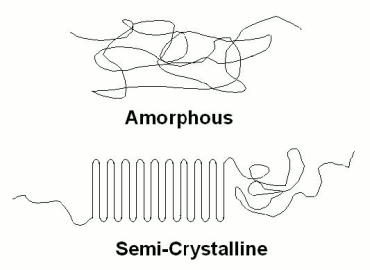
\includegraphics[width=0.4\textwidth]{fig/crystal-1.png}
    \caption{Как цепочки складываются в ламели}
    \label{fig:crystal-1}
  \end{center}
  \vspace{-20pt}
  \vspace{1pt}
\end{wrapfigure}



\begin{figure}[h]
    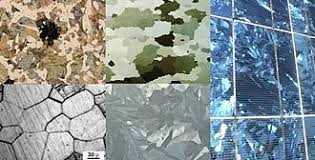
\includegraphics[width=\textwidth]{fig/crystallites.jpg}
    \caption{Типы кристаллитов}
    \label{fig:crystallites}
\end{figure}



\subsection{Частичная кристалличность}

	
	\begin{wrapfigure}{r}{0.5\textwidth} 
\vspace{-20pt}
  \begin{center}
    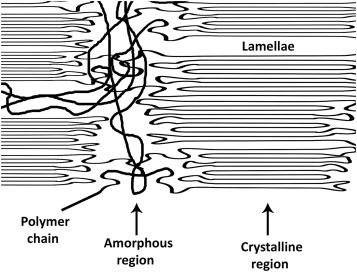
\includegraphics[width=0.4\textwidth]{fig/crystal-2.jpg}
    \caption{К определению кристалличности полимеров}
    \label{fig:crystal-2}
  \end{center}
  \vspace{-20pt}
  \vspace{1pt}
\end{wrapfigure}	

\subsection{Влияние на макроскопические параметры}

\section{Исследование кристаллической структуры}
\subsection{ЯМР}
\subsection{Еще что-то}
\subsection{Сравнение и обоснование}
тут методы, обоснование

\section{Исследование структуры с помощью дифракции рентгеновского рассеяния}

\subsection{Синхротронное излучение}
когерентные источники, йоу!
\subsection{Упругое рассеяние}
\subsection{2D-снимки, порошковая дифракция}
\subsection{Неупругое рассеяние,гало}
эффекты от аморфной части



	